\section{Overview}

To motivate our approach, consider how we might test a highly simplified
model of a distributed key-value database application, depicted
in \autoref{fig:database}.

\begin{figure}[ht!]
    \centering
    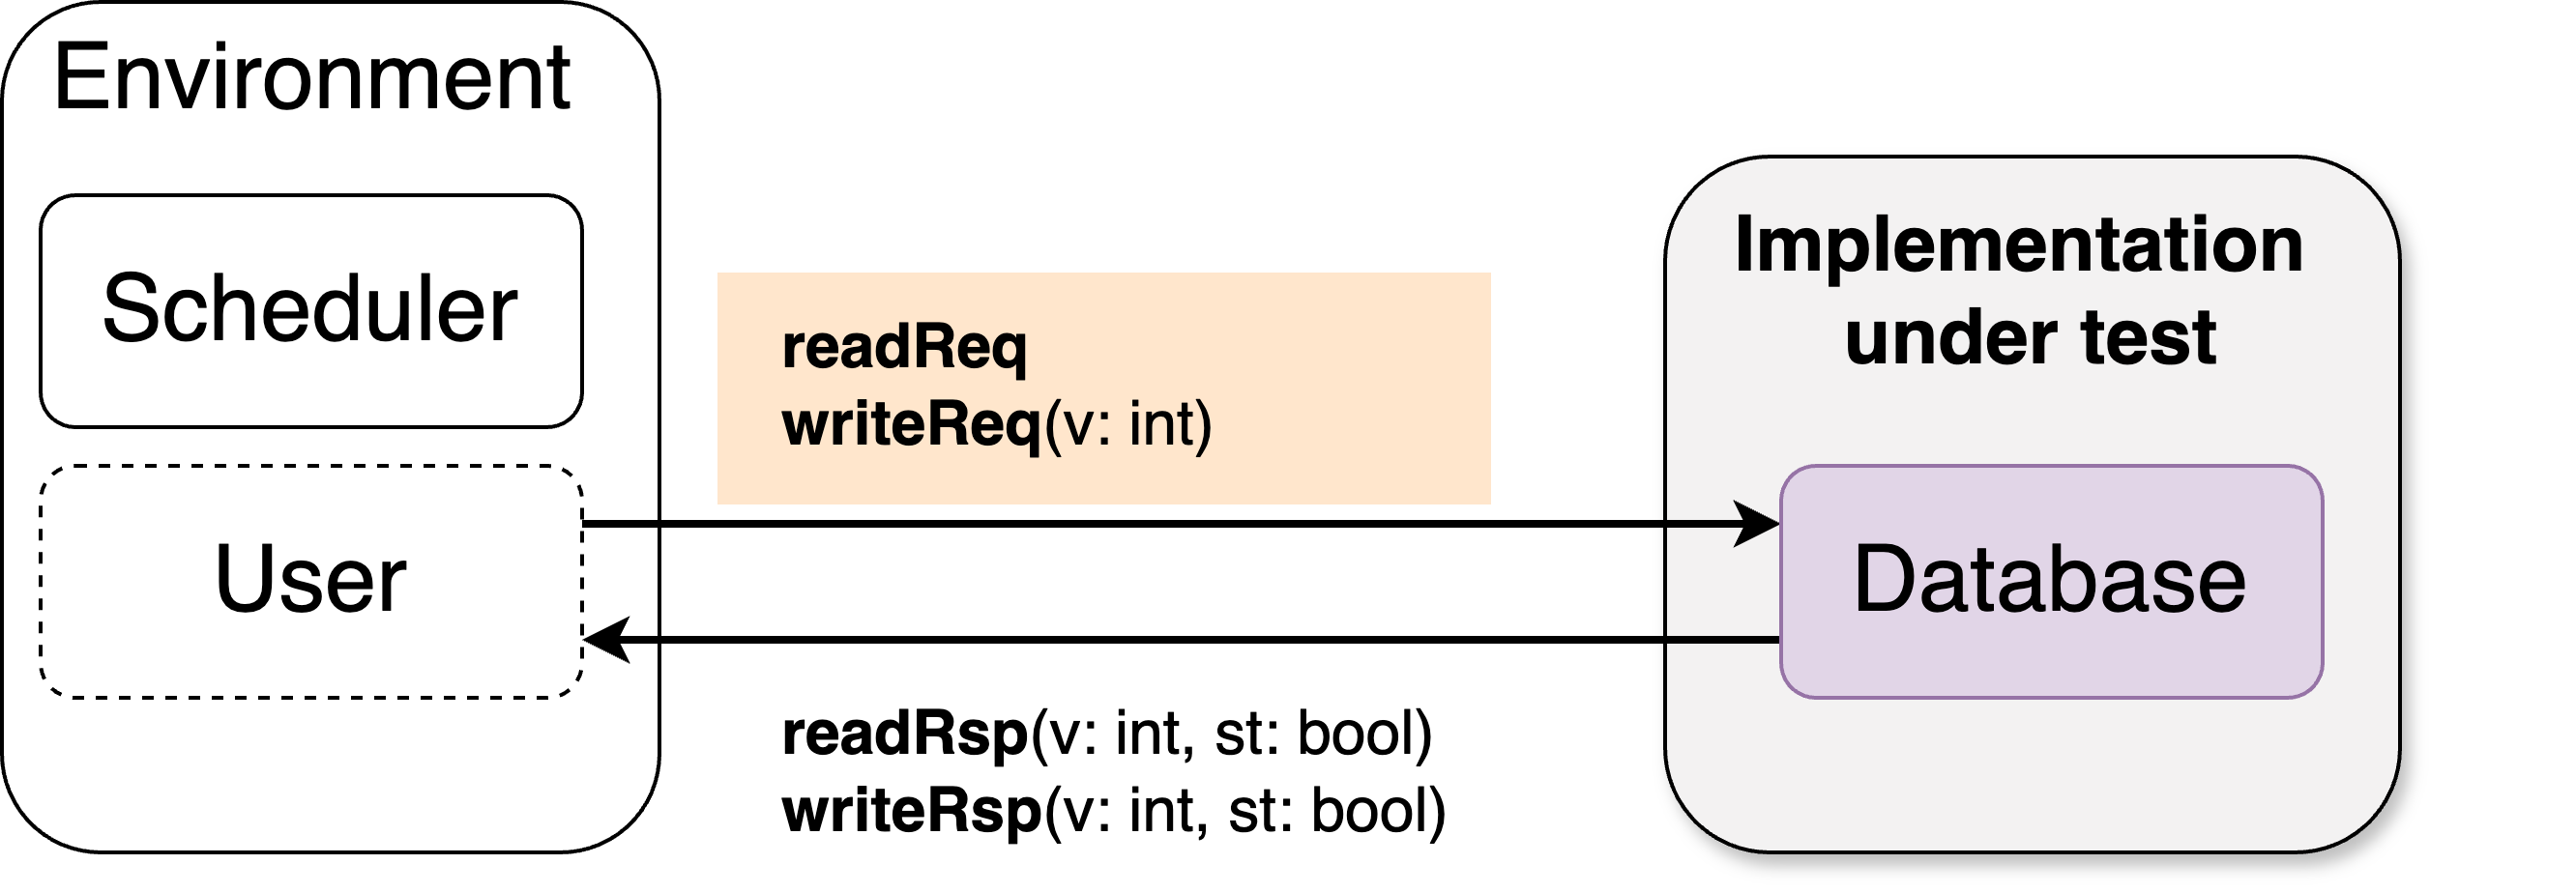
\includegraphics[width=0.65\linewidth]{figures/readWrite.drawio-simp.png}
    \caption{A simplified database access workflow.}
    \label{fig:database}
\end{figure}

This system includes two components: a user that models input
generation of messages that read and write to a model of a database
under test, and the database itself that is responsible for persisting
writes generated by users, and responding to requests to read its
contents.  To simplify this structure, we assume the database manages
exactly one key and users simply perform requests to read that key or
write new values to it; the key argument is therefore elided in our
specifications.  As discussed earlier, reads and writes to the
database are asynchronous and separated into two event classes, one
that models requests and the other that models responses to previously
issued requests.  Each response carries a status flag indicating if
the request was successful.  A \textsf{true} status value on a
$\eff{writeRsp}$ message indicates that an earlier corresponding request
was successfully persisted to the database, while a \textsf{true}
status flag on a $\eff{readRsp}$ message indicates that the database is
not empty, and the value returned reflects the effect of a previous
write.

Since our focus in this paper is on deriving a controller that
schedules messages and determines payloads to drive a testing
procedure, we are unconcerned with how the implementation of the
database is precisely modeled - our primary interest is in the
specification of its interface and the dependencies that must hold on
messages sent between the users and the database, since these are the
primary elements that inform scheduling decisions.  The goal of the
synthesized controller generates user requests and orders the delivery
of messages in an attempt to drive execution to a violation of some
safety property we wish to establish about the system.

In the figure, $\eff{readReq}$ and $\eff{writeReq}$ messages (marked
in orange) sent by the user do not depend on any prior messages or
actions taken by other components. We refer to such messages as
directly \emph{generatable}. In contrast, messages sent from the
database back to to the user are \emph{observable} - their order and
contents depend upon previously issued messages.

\paragraph{Traces and safety}
An executable model, provided user inputs, generates a sequence of
messages with concrete values as payloads, which we refer to
as a \emph{trace}.  In this example, we consider a weaker safety
property than strong consistency as discussed in the previous section.
Here, we expect the database to satisfy a \emph{read-your-writes} (RYW)
consistency policy~\cite{...}  in which reads see the most recent
write to the database.  Under a database that provides only weak
eventually consistent semantics, however, we might witness the
following trace:
{\small\begin{align*} tr_1 \doteq
  &\effGreen{writeReq(3)};\effBlue{writeReq(4)};\effBlue{writeRsp(4,\true)};\effRed{readReq};\effGreen{writeRsp(3,\true)};\effRed{readRsp(4,
    \true)}
\end{align*}}\noindent
Here the value returned by the $\effRed{readRsp}$ generated as a
result of a previously issued $\eff{readReq}$ returns a value that is
not the most recent one in the database.  This can happen, for
example, if the database is replicated and the effect of the
$\effGreen{writeRsp(3,true)}$ event is not propagated to all replicas,
one of which responds to the $\effRed{readReq}$ event.

We can formally express a violation of RYW as the following specification,
defined as a symbolic LTL$_f$ formula~\cite{...}:
{\footnotesize\begin{align*} \negSCA
    \doteq \finalA (\msg{writeRsp}{v = \Code{x} \land st = \true}
    \land (\neg \msg{writeRsp}{st = \true}) \untilA \msg{readRsp}{v =
      \Code{y} \land \Code{y} \not= \Code{x}})
\end{align*}}\noindent
Here, $\msg{writeRsp}{v = \Code{x} \land st = \true}$ represents an
atomic predicate for a message, referred to as a \emph{symbolic
  event}. This indicates that the message constructs a
$\eff{writeRsp}$ event with $\Code{x}$ as the write value (i.e., field
$v$) and a $\true$ status (i.e., field $st$) as its payload. We use
the standard LTL final modality $\finalA$ and the until modality
$\untilA$ to express temporal dependencies. The formula reads: "there
will \emph{eventually} be a successful $\eff{writeRsp}$ message with
the write value $\Code{x}$, and moreover, there will be no subsequent
successful $\eff{writeRsp}$ message (i.e., $\Code{x}$ is the last
write value) \emph{until} an $\eff{readRsp}$ message with a payload
$\Code{y}$ different from $\Code{x}$ occurs."  This formula can be
transformed into Symbolic Finite Automata (SFA)~\cite{...}, which
provides a decidable procedure for inclusion and emptiness checks. It
is important to note that this specification defines an
overapproximation of violating traces.  Thus, not all traces
consistent with this property property are necessarily realizable. For
example, although the trace
$\effGreen{writeRsp(3,\true)};\effBlue{readRsp(-1,\true)}$ is consistent
with (aka satisfies) $\negSCA$, it does not represent a realizable
execution because it does not contain corresponding request messages
for the write and read.

\begin{figure}
    \centering
\begin{minted}[xleftmargin=5pt, numbersep=4pt, linenos = true, fontsize = \footnotesize, escapeinside=??]{OCaml}
?$\mykw{assert}$? (x != y); 
?$\mykw{gen}$? ?$\eff{writeReq}$? x;
?$\mykw{gen}$? ?$\eff{writeReq}$? y;
let (y1: int) (s1: bool) = ?$\mykw{obs}$? ?$\eff{writeRsp}$?; ?$\mykw{assert}$? (y1 == y && s1 == true);
?$\mykw{gen}$? ?$\eff{readReq}$?;
let (x1: int) (s2: bool) = ?$\mykw{obs}$? ?$\eff{writeRsp}$?; ?$\mykw{assert}$? (x1 == x && s2 == true);
let (y2: int) (s3: bool) = ?$\mykw{obs}$? ?$\eff{readRsp}$?; ?$\mykw{assert}$? (y2 == y && s3 == true)
\end{minted}
    \caption{A controller $P_{C}$ that is consistent with $\negSCA$. }
    \label{fig:2pc-term}
\end{figure}

\paragraph{Controllers}
As mentioned earlier, testing the components in reactive a distributed
system requires the support of a controller.  We introduce a DSL for
expressing controllers. A controller program manages the generation of
messages, schedules message order, and constrains data dependencies
between messages.  Concretely, to realize the trace $tr_1$ given
above, the controller must provide generatable messages (e.g.,
$\effGreen{writeReq(3)}$).

A controller program $P_{C}$ that generates traces geared towards
exhibiting the violation property specified by $\negSCA$ is shown in
\autoref{fig:2pc-term}. The program's body defines a message ordering
using the keywords $\mykw{gen}$ and $\mykw{obs}$, which indicate
whether the message is directly generated by the user or
the database (i.e., the system-under-test).  It is also
the controller's responsibility to provide the payload for generatable
messages, and it can bind the payloads of observable messages to new
variables. The constraints on parameters $\Code{x}$ and $\Code{y}$ are
defined by the $\mykw{assert}$ statements on lines 1.  Since the
controller does not control the internal behavior of components, it
cannot directly enforce specific traces; in other words, it cannot
mandate the specific values output by the database in response to a
message. Instead, it uses assertions to guide the execution towards
traces consistent with $\negSCA$.  However, assertions may fail; for
instance, if the database component sends a $\eff{writeRsp}$ message
with a $\false$ status, this would violate the assertion on line 4.
Nonetheless, our synthesis procedure guarantees that it will generate
an execution of the system that produces the expected traces in
$\negSCA$, if one exists.  

% {\footnotesize\begin{align*}
%     &\Code{readReq}: \Code{unit} \quad& \Code{readRsp}: va\hasnty{int} \sarr \Code{unit}
%     \\&\Code{getReq}: \Code{unit} \quad&
%     \Code{getRsp}: va\hasnty{int} \sarr \Code{unit}
%     \\&\Code{writeReq}: va\hasnty{int} \sarr \Code{unit} \quad&
%     \Code{writeRsp}: va\hasnty{int} \sarr st\hasnty{bool} \sarr \Code{unit}
%     \\&\Code{putReq}: va\hasnty{int} \sarr \Code{unit} \quad&
%     \Code{putRsp}: va\hasnty{int} \sarr st\hasnty{bool} \sarr \Code{unit}
%     \\&\Code{commit}: va\hasnty{int} \sarr \Code{unit} \quad&
%     \Code{Abort}: \Code{unit}
% \end{align*}}

\subsection{Prophecy Automata Types}

\newcommand{\specRealizable}{A_\Code{realizable}}

For a given violation property (e.g., $\negSCA$), when we have no assumptions about component behaviors, all traces accepted by $\negSCA$ are worth exploring, including clearly unrealizable traces such as $\effGreen{writeRsp(3,\true)};\effBlue{readRsp(-1,\true)}$, as noted previously.
To filter out these unrealizable traces, we need specifications for components that establish necessary message relation in realizable traces. These specifications are both temporal (e.g., response messages should follow corresponding request messages) and data-dependent (e.g., the payload of a read response should match the most recent write value). On the other hand, they should also align with the actual implementation of the reactive system. Unlike defining a violation property, crafting an s-LTL$_f$ property $\specRealizable$ to capture all realizable traces precisely is non-trivial, as different messages are handled by different nodes in distributed system.

To achieve both expressiveness and compositionality, we use trace-based refinement types \cite{...} to constrain each message handler, instead of provide a global specification. In this approach, the reactive system is modeled as a set of function types, where each function name corresponds to a message name, parameter types define constraints on message payloads, and return types specify relationships between messages.
Unlike standard trace-based refinement types, our model incorporates asynchronous semantics, where handling one message can trigger the sending of new messages that will only be received later. Thus, return types must include both a ``rely", specifying assumptions about prior events, and a ``guarantee", constraining future events. Based on this, we introduce Prophecy Automata Types (\PAT), which act as a ``prophecy" to constrain which messages should be received in the future.

% While reachability properties are naturally expressed using s-LTL$_f$
% and SFA, the behavior of a plan program cannot be directly captured by
% standard temporal logic due to the interaction between the environment
% and the components it orchestrates.  These components, such as the
% coordinator in the two-phase commit (2PC) example, can be seen as a
% set of message handlers (effectful functions). For example, the
% coordinator handles messages like $\eff{readReq}$, $\eff{writeReq}$,
% $\eff{getRsp}$, and $\eff{putRsp}$ (i.e., all input messages directed
% at the coordinator, as shown in \autoref{fig:2pc-workflow}). These
% handlers are stateful, meaning their current behavior is dependent on
% previously occurred events.  Furthermore, due to the asynchronous
% nature of reactive systems, the result of one handler’s computation is
% not immediately observable. Instead, it materializes as a newly sent
% message, which may only be received at some future point. For example,
% the handler of a $\eff{getReq}$ message sends a $\eff{getRsp}$ message
% containing the read value as its payload. This read value is not
% arbitrary—it is the last value that was successfully $\eff{commit}$ed
% in the past. This dynamic nature, where message handlers both depend
% on past events and propagate their effects into the future, push us
% introduce the Prophecy Automata Type (PAT).


\begin{figure}[ht!]
    \centering
{\footnotesize\begin{align*}
    \eff{writeReq}:&  \Code{x}\hasnty{int} \sarr \rg{\allTL}{\lastA\msg{writeReq}{v = \Code{x}}}{\finalA\msg{writeRsp}{v = \Code{x}}}
    \\\eff{writeRsp}:& \Code{x}\hasnty{int} \sarr \Code{s}\hasnty{bool} \sarr \rg{\allTL}{\lastA\msg{writeRsp}{v = \Code{x} \land st = \Code{s}}}{\allTL}
    \\
    \\\eff{readReq}:&  \Code{x}\hasnty{int}\garr \rg{\finalA \msg{writeReq}{v = \Code{x}} \land \neg\nextA\finalA\msg{writeReq}{\top}}{\lastA\msg{readReq}{\top}}{\finalA\msg{readRsp}{v = \Code{x} \land st}}
    \\&\interty  \rg{\neg\finalA \msg{writeRsp}{\top}}{\lastA\msg{readReq}{\top}}{\finalA\msg{readRsp}{ \neg st}}
    \\\eff{readRsp}:& \Code{x}\hasnty{int}\sarr \Code{s}\hasnty{bool} \sarr \rg{\allTL}{\lastA\msg{readRsp}{v = \Code{x} \land st = \Code{s}}}{\allTL}
\end{align*}}
    \caption{Components Specification $\Delta$ that is expressed in Prophecy Automata Type (\PAT) of messages }
    \label{fig:2pc-pat}
\end{figure}

\paragraph{History, current, and prophecy automata} The message specification $\Delta$ of reactive system in our motivating example is shown in \autoref{fig:2pc-pat}, where we still use s-LTL$_f$ to express SFAs in \PAT{}s. The return type of these messages has the form $\rg{H}{A}{F}$, where $H$, $A$, and $F$ represent the history, current, and prophecy automata, respectively. It means that: ``If a program is executed under a context trace accepted by the history automaton $H$, then the execution will produce a present trace accepted by the current automaton $A$, moreover, the future trace (the remaining part of the execution) will be accepted by the prophecy automaton $F$''. In this sense, prophecy automata serve as the trace-based analogue of prophecy variables\cite{...}, which have been introduced in other state-based concurrency reasoning approaches. For example, the first type in \autoref{fig:2pc-pat} is about $\eff{writeReq}$ and has history automaton that allows $\eff{writeReq}$ to be received at any context, i.e., any messages ($\evparenth{\top}$) are allowed within the context trace globally ($\globalA$). The current automaton only allows singleton ($\lastA$ modality in s-LTL$_f$) trace with message $\eff{writeReq}$ itself. This is consistent that the handling of message $\eff{writeReq}$ can only make itself happens. More interestingly, the prophecy automaton guarantees that in the future a $\eff{writeRsp}$ message will be handled in the future, since the handler of $\eff{writeReq}$ will send a $\eff{writeRsp}$ message that is expected to be received in the future following the asynchronous semantics.

\paragraph{Control flows} The history, current, and prophecy automata can describe the control follows  of the message handler. For example, the type of $\eff{readReq}$ use intersection type ($\interty$) encodes two situations the handler may face, i.e., wether there exists a previous write value. The first type indicates the handler of message $\eff{readReq}$ should send the written value ($\Code{x}$ in $\msg{writeReq}{v = \Code{x}}$) which is also the last one ($\nextA\finalA\msg{writeReq}{\top}$) as an response message ($\msg{readRsp}{v = \Code{x} \land st}$) with $\true$ status. Otherwise, there is no write value ($\neg\finalA \msg{writeRsp}{\top}$), then the a $\eff{readRsp}$ with a $\false$ status ($\finalA\msg{readRsp}{ \neg st}$) should be received in the future. On the other hand, the handlers of observable messages $\eff{readRsp}$ and $\eff{writeRsp}$ are exactly the controller (user) itself. Thus, the prophecy automata of these types has not guarantee about future ($\allTL$), since we cannot constrain what message will be sent by user.

% This structure allows for a more nuanced reasoning about asynchronous message-passing systems, where both past and future events are connected with current events. The inclusion of prophecy automata adds flexibility in reasoning about future states in a way that traditional two-state specification (pre- and post-condition based) cannot, making it particularly suited to reactive systems.

% \begin{example}[message specification] The specification of the coordinator and database components in the 2PC example is shown in \autoref{fig:2pc-pat}, represented as two groups of message types. Messages are treated as effect operators and are denoted by function refinement types, where the automata in these types are still expressed in s-LTL$_f$. 
% Since each message handling contributes exactly one event to the trace, the present automaton is always a singleton event, denoted by the standard $\lastA$ modality in s-LTL$_f$. The dependencies between messages are captured by the $\rg{H}{A}{F}$ triple.
% For instance, the first type in \autoref{fig:2pc-pat} specifies that handling the $\eff{readReq}$ message results in sending a new message $\eff{getReq}$. In other words, a new event $\eff{getReq}$ will occur in the future ($\finalA \msg{getReq}{\top}$). The type of $\eff{getReq}$ consists of two cases, connected using an intersection type ($\interty$).
% The first case indicates a $\eff{readRsp}$ message will eventually be triggered, with its payload equal to the last committed value (i.e., $\finalA \msg{commit}{va = x} \land \neg\nextA\finalA\msg{commit}{\top}$). This is expressed with the help of a ghost variable to link the last committed value in history automata into prophecy automata. The second case handles the situation where no committed value exists, then reads default value ($-1$).
% \end{example}

\paragraph{Type check over \PAT} By defining message specification as function \PAT over messages, we can perform standard refinement type check on the controller programs to decide if they are consistent of the message specification. In this sense, all $\mykw{gen}$ and $\mykw{obs}$ terms in the controller program are treated as function application, which should be consistent with the function \PAT of corresponding message in message specification $\Delta$.
For example, the controller $P_{C}$ is type-safe, where a observed $\eff{readReq}$ term on line $5$ in \autoref{fig:2pc-term} can divide the whole program intro three pieces: history pieces (line $1$ - $4$), current piece (line $5$), and future piece (line $6$ - $7$). These three piece are consistent with the first case of \PAT of $\eff{readReq}$, which requires the last write value is $\Code{y}$ (line $3$) in the history, current handling message is $\eff{readReq}$, and there will be a success $\eff{readReq}$ with value $\Code{y}$ in the future (line $7$). Moreover, the controller $P_{C}$ can indeed induce a trace that violate the RYW consistency policy. This is be also proved by type check controller $P_{C}$ against a \PAT $\rg{\globalA\evparenth{\bot}}{\negSCA}{\globalA\evparenth{\bot}}$, which assume there is no history message happens ($\globalA\evparenth{\bot}$), the execution of controller generate trace consistent with $\negSCA$, and also not more pending message to be received in the future ($\globalA\evparenth{\bot}$).

\subsection{Controller Program Synthesis}

\begin{figure}[ht!]
    \centering
    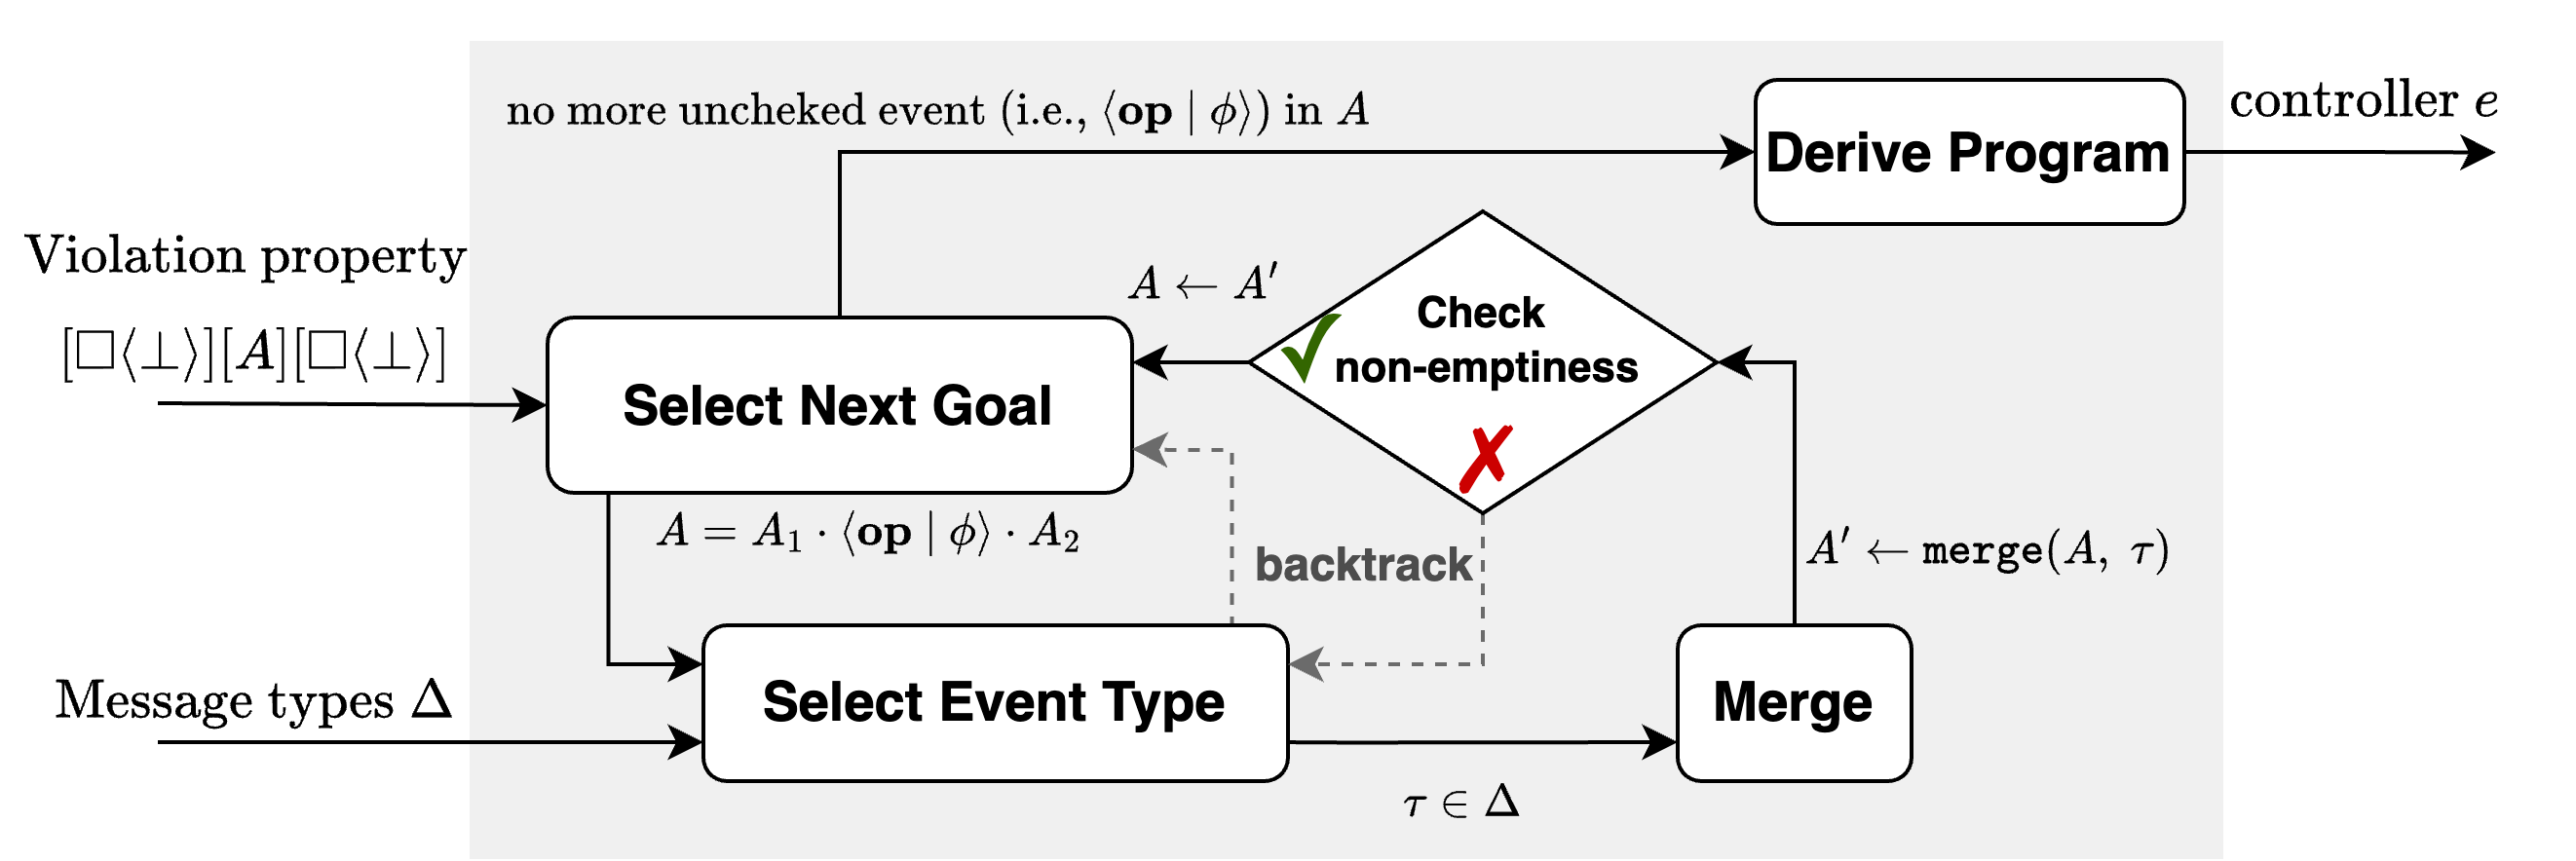
\includegraphics[width=0.95\linewidth]{figures/intuition-plan-syn.drawio.png}
    \caption{Intuition of synthesis algorithm}
    \label{fig:intuition-algo}
\end{figure}

% For example, desirable controller should uses messages properly with respect to message specification $\Delta$, moreover, can be type checked against \PAT $\rg{\globalA\evparenth{\bot}}{\negSCA}{\globalA\evparenth{\bot}}$.

By treating messages as library methods, controller program synthesis can be formalized as a type-guided, component-based synthesis task, where the types of library methods are provided by message specifications $\Delta$. Naive enumeration of these message invocations is impractical due to exponential complexity. Instead, our algorithm incrementally refines the violation property to exclude unrealizable traces.
As illustrated in \autoref{fig:intuition-algo}, our algorithm consists of two parts. First, it refines the violation property $A$ to $A'$, where $A' \impl A$, ensuring all message invocations in $A'$ align with $\Delta$. Second, it derives the corresponding plan program from $A'$. For instance, the refined property of $\negSCA$ in our motivating example can be:
{\footnotesize\begin{align*}
\negSCA
    \equiv
    &\anyA^* \seqA \textcolor{DeepGreen}{\msg{writeRsp}{v = \Code{x} \land st}} \seqA
    (\anyA \setminus \msg{writeRsp}{ st})^* \seqA
    \textcolor{red}{\msg{readRsp}{v = \Code{y} \land st \land v \not= \Code{y}}} \seqA \anyA^* \tag{desugar into SRE}
\\\negSCA'
    \doteq
    &\msg{writeReq}{v = \Code{x}} \seqA
    \msg{writeReq}{v = \Code{y} \land v \not= \Code{x}} \seqA
    \msg{readReq}{\top} \seqA
    \\&\msg{writeRsp}{v = \Code{y} \land st} \seqA
    \textcolor{DeepGreen}{\msg{writeRsp}{v = \Code{x} \land st}} \seqA
    \textcolor{red}{\msg{readRsp}{v = \Code{y} \land st \land v \not= \Code{x}}}
\end{align*}}\noindent
To emphasize that all traces consistent with $\negSCA'$ also satisfy $\negSCA$, we highlight two key symbolic events, $\effGreen{writeRsp}$ and $\effRed{readRsp}$, which violate the Read-Your-Writes (RYW) consistency policy.
As shown, the property $\negSCA'$ closely resembles the controller program $P_{C}$. The main difference is that $P_{C}$ is more operational, divides messages into $\mykw{gen}$ (generatable) and $\mykw{obs}$ (observable) groups. The controller provides payloads for $\mykw{gen}$ messages, while payloads in $\mykw{obs}$ messages are constrained only by local variables.

% Then, by properly instantiate variables in $\negSCA'$

% The first part refines the violation property $A$ (e.g., $\negSCA$) into a $A'$ where $A' \impl A$ such that all message invocations in $A'$ are consistent with $\Delta$. 

% The second part derives the corresponding plan program from $A'$.
% The first part is the most crucial, as it needs to adapt PAT to constrain the local message invocations within property $A$ that is in a global view.


% On the other hand, the set of plan programs that are consistent with the reachability property $A$ can be defined as those programs that have the type $\rg{\epsilon}{A}{\epsilon}$. This type indicates that the plan program starts with an empty history trace and does not need to guarantee any further future events to be happened. 
% Thus, a desirable plan program is one that resides in the "intersection" of programs consistent with both the message specification $\Delta$ and the reachability property $A$. 
% Finding such a plan program can be formalized as a type-driven synthesis problem, i.e., search a plan program that has the type $\rg{\epsilon}{A}{\epsilon}$, where the message types are provided in the message specification $\Delta$. 
% The naive component-based enumeration of these message invocation cannot solve this synthesis problem since it would suffer from exponential complexity.  Therefore, a more efficient synthesis algorithm should combine the specifications from both $\Delta$ and $A$ intelligently. 

% The intuition behind our synthesis algorithm is illustrated in \autoref{fig:intuition-algo}. As previously discussed, the essence of synthesizing a plan program lies in finding the "intersection" of behaviors permitted by both the message specifications $\Delta$ and the reachability property $A$. To operationalize this idea, our algorithm is structured into two main parts. The first part refines the property $A$ into a subset $A'$ (where $A' \subseteq A$) such that all message invocations in $A'$ are consistent with $\Delta$. The second part derives the corresponding plan program from $A'$.


\paragraph{Property Refinement Loop} 
The property refinement process is crucial, as it adapts \PAT to constrain all messages in the refined property $\negSCA'$. Although $\negSCA'$ includes $6$ events, not all (e.g., $\eff{readReq}$) are directly found in the original $\negSCA$. The algorithm dynamically add new messages that need to be check as subgoal when it solving one subgoal.
For example, when checking the type of the $\eff{readRsp}$ message, the last message in $\negSCA$ (highlighted in red), the algorithm identifies that $\eff{readRsp}$ is sent by the handler for $\eff{readReq}$ (via the type of $\eff{readReq}$). Moreover, the type of $\eff{readReq}$ also indicates the payload $\Code{y}$ of $\eff{readRsq}$ should belong to a previous $\eff{writeReq}$.
It then adds $\eff{writeReq}$ and $\eff{readReq}$ before $\eff{readRsp}$ in the refined property, also marking them as messages to be checked later.
{\footnotesize\begin{align*}
\negSCA''
    \doteq
    &\anyA^* \seqA \msg{writeReq}{v = \Code{y}} \seqA \anyA^* \seqA \msg{readReq}{\top} \seqA \anyA^* \seqA
    \\&\textcolor{DeepGreen}{\msg{writeRsp}{v = \Code{x} \land st}} \seqA
    (\anyA \setminus \msg{writeRsp}{ st})^* \seqA
    \textcolor{red}{\msg{readRsp}{v = \Code{y} \land st \land v \not= \Code{y}}} \seqA \anyA^* \tag{after check $\eff{readRsp}$}
\end{align*}}\noindent

To achieve this, we construct a refinement loop, as shown in \autoref{fig:intuition-algo}. In each loop iteration, the algorithm selects a unsolved symbolic event $\msg{op}{\phi}$ from property $A$. Then, it selects a type $\tau$ from $\Delta$ for the operator $\eff{op}$ and merges it with $A$.
To ensure the synthesized controller can realize at least one execution, the merged result ($A'$) must contain at least one trace, which the diamond box in \autoref{fig:intuition-algo} verifies using a standard SFA non-emptiness check. If $A'$ is non-empty, the refinement loop continues; if it is empty, the algorithm backtracks to try a different type from $\Delta$ or chooses another subgoal. This loop ends when all symbolic events in $A$ (except those within Kleene star expressions) are verified consistent with $\Delta$.
{\footnotesize\begin{align*}
    &\anyA^* \seqA \msg{writeReq}{v = \Code{x}} \seqA \anyA^* \seqA
    \msg{writeReq}{v = \Code{y} \land v \not= \Code{x}} \seqA \anyA^* \seqA
    \msg{readReq}{\top} \seqA \anyA^* \seqA
    \\&\msg{writeRsp}{v = \Code{y} \land st} \seqA \anyA^* \seqA
    \textcolor{DeepGreen}{\msg{writeRsp}{v = \Code{x} \land st}} \seqA (\anyA \setminus \msg{writeRsp}{ st})^* \seqA
    \textcolor{red}{\msg{readRsp}{v = \Code{y} \land st \land v \not= \Code{x}}} \anyA^*
\end{align*}}\noindent
Our algorithm choose shorter programs that satisfy the violation property; thus, it specializes all Kleene stars to $\epsilon$, resulting in the final refined property.

Viewed from another perspective, our approach functions as a trace-exploration algorithm, exploring traces consistent with violation property until one align with $\Delta$. The primary challenge lies in handling the Kleene star, which allows for arbitrary unrolling. The algorithm in \autoref{fig:intuition-algo} takes a lazy approach, unrolling the Kleene star only as necessary. For instance, refining $\negSCA$ to include an additional $\eff{writeReq}$ and $\eff{readReq}$ results in $\negSCA'$ by forcing the first $\anyA^*$ in $\negSCA$ to refine as $\anyA^* \seqA \msg{writeReq}{v = \Code{y}} \seqA \anyA^* \seqA \msg{readReq}{\top} \seqA \anyA^* \seqA$, which also unrolls the Kleene star.

The details of algorithm will explained in \autoref{sec:algo}.

% In another perspective, our approach can be treat as a smart trace exploring algorithm, i.e., where we explore traces that included by violation property, and until it is consistent with $\Delta$. The most difficult part is dealing the Kleene star, which may lead arbitrary times of unrolling. Then, the algorithm in \autoref{fig:intuition-algo} takes a lazy manner, which means the Kleene star is unrolled by need. For example, the property $\negSCA'$ that is result of inserting a $\eff{readReq}$ into $\negSCA$, which force the first $\anyA^*$ in $\negSCA$ to be refined into $\anyA^* \seqA \eff{readReq} \seqA \anyA^*$.

% \paragraph{Searching heuristic} There are two key intuitions:
% \begin{enumerate}
%     \item Focusing: if we doesn't finish one causal group of messages (e.g., messages for read operation that are colored in blue), we should not switch into another group of messages.
%     \item Backward to root: we always first use backward synthesis to find the generatable message that is the ``root'' of one operation, then perform forward synthesis.
% \end{enumerate}

% \begin{example}[Synthesis] 
% We will explain how our synthesis algorithm operates using our motivating example. For clarity, we represent both the property and PATs using desugared SFA in the form of Symbolic Regular Expressions (SRE). Initially, the desugared property $A$ is defined as follows:
% {\footnotesize\begin{align*}
%     A \doteq \anyA^* \seqA \msg{writeRsp}{va = \Code{x} \land stat = \true} \seqA (\anyA \setminus \msg{writeRsp}{stat = \true})^* \seqA \msg{readRsp}{va = \Code{y} \land \Code{y} \not= \Code{x}} \seqA \anyA^*
% \end{align*}}\noindent
% Assume we select the message $\eff{readRsp}$ from $A$ and choose to perform a backward synthesis, we can identify the corresponding type $\tau_\Code{getRsq}$ in $\Delta$ as following:
% {\footnotesize\begin{align*}
%     \eff{getRsp}:& x\hasnty{int}\sarr \rg{\allTL}{\lastA\msg{getRsp}{va = x}}{\finalA\msg{readRsp}{va = x}} \tag{$\tau_\Code{getRsq}$}
%     \\& x\hasnty{int}\sarr \rg{\anyA^*}{\msg{getRsp}{va = x}}{\anyA^* \seqA \msg{readRsp}{va = x} \seqA \anyA^*} \tag{after desugar}
% \end{align*}}\noindent
% whose prophecy automata ($\anyA^* \seqA \msg{readRsp}{va = x} \seqA \anyA^*$) indicate that a read response is expected to occur in the future. After merge $A$ with $\tau_\Code{getRsq}$, the one possible merged result $A'$ will assume there is $\eff{getRsp}$ message with the same payload happens before $\eff{readRsp}$.
% {\footnotesize\begin{align*}
%     A' \doteq &\anyA^* \seqA \msg{writeRsp}{va = \Code{x} \land stat = \true} \seqA (\anyA \setminus \msg{writeRsp}{stat = \true})^* \seqA \textcolor{red}{\msg{getRsp}{va = x}} 
%     \\& (\anyA \setminus \msg{writeRsp}{stat = \true})^* \seqA \msg{readRsp}{va = \Code{y} \land \Code{y} \not= \Code{x}} \seqA \anyA^*
% \end{align*}}\noindent
% Easily know $A'$ is not empty automata. Then, the $\eff{getRsp}$ is colored red to to signify that it has already been verified, indicating that the events before and after $\eff{getRsp}$ are already consistent with type $\tau_\Code{getRsq}$ from $\Delta$.
% This process is termed backward synthesis, as the new event $\eff{getRsp}$ is introduced prior to $\eff{readRsp}$. 
% The backward synthesis will continue until we face the generatable message. For example, $\eff{getRsp}$ is actually triggered by another event $\eff{getReq}$, and finally triggered by the generatable message $\eff{readReq}$. 

% On the other hand, we can also preform forward synthesis at $\eff{readRsp}$, which involves directly merging $A$ with the type of $\eff{readRsp}$. Since the receiver $\eff{readRsp}$ is user (environment), thus it won't trigger any new message and omitted from \autoref{fig:2pc-pat}. Thus, it will have type
% {\footnotesize\begin{align*}
%     \eff{readRsp}:& x\hasnty{int}\sarr \rg{\allTL}{\lastA\msg{readRsp}{va = x}}{\allTL}
%     \\& x\hasnty{int}\sarr \rg{\anyA^*}{\msg{readRsp}{va = x}}{\anyA^*} \tag{after desugar}
% \end{align*}}\noindent
% which induce a merged result $A''$ shown below.
% {\footnotesize\begin{align*}
%     A'' \doteq &\anyA^* \seqA \msg{writeRsp}{va = \Code{x} \land stat = \true} \seqA (\anyA \setminus \msg{writeRsp}{stat = \true})^* \seqA \textcolor{red}{\msg{getRsp}{va = x}} 
%     \\& (\anyA \setminus \msg{writeRsp}{stat = \true})^* \seqA \textcolor{red}{\msg{readRsp}{va = \Code{y} \land \Code{y} \not= \Code{x}}} \seqA \anyA^*
% \end{align*}}\noindent

% It is important to note that the Kleene star in property $A$ can be straightforwardly underapproximated to $\epsilon$ automata. Consequently, the processes of backward and forward synthesis conclude once all symbolic events that are not encapsulated within the Kleene star have been resolved (indicated in red). As a result, one potential refinement of the automaton can be represented as follows:
% {\footnotesize\begin{align*}
%     &\msg{writeReq}{va = \Code{x}}\seqA \msg{putReq}{va = \Code{x}}\seqA \msg{putReq}{va = \Code{x} \land stat = \true}\seqA \msg{writeRsp}{va = \Code{x} \land stat = \true} \seqA 
%     \\&\msg{readReq}{\top} \seqA \msg{getReq}{\top} \seqA \msg{getRsp}{va = \Code{y} \land \Code{y} = -1} \seqA \msg{readRsp}{va = \Code{y} \land \Code{y} \not= \Code{x}} \seqA \msg{readRsp}{va = \Code{y} \land \Code{y} \not= \Code{x}} \seqA
%     \\&  \msg{commit}{va = \Code{x}}
% \end{align*}}\noindent
% which can derive a plan program $e_{P_1}$ shown in \autoref{fig:2pc-term}.
% \end{example}

